\usepackage[ngerman, english]{babel}


\title{Anti-Aging: State of the Art}
\author{Felix Karg}


\graphicspath{ {./img/} {../template/} {../template_tex/} } % add further graphics paths here

\newif\iftwocols
\twocolsfalse
% \twocolstrue


\usepackage{etex}
\usepackage{graphicx}
\usepackage[export]{adjustbox}
\usepackage{multicol}
\usepackage{pdfpcnotes}
\usepackage{pdfpages}
% \usepackage[dvipsnames]{xcolor}


% \usepackage{minted}
% \usemintedstyle{pastie}


\usetheme[numbering=fraction, progressbar=frametitle]{metropolis}


\date{December 29, 2020}
% \date{12. Juli 2019}


% \institute{Add Your Institute here}
% \titlegraphic{\vspace{4cm} \hspace{7cm} \includegraphics[height=2cm]{Logo_INST}}
% \titlegraphic{\vspace{4cm} \hspace{7cm} \Huge\LaTeX}

\iftwocols
\AtBeginSection[]
{
    \large
    \begin{frame}{Agenda}
        \begin{multicols}{2}
            \tableofcontents[currentsection]
        \end{multicols}
        \clearpage
    \end{frame}
}

\AtBeginSubsection[]
{
    \large
    \begin{frame}{Agenda}
        \begin{multicols}{2}
            \tableofcontents[currentsection,currentsubsection]
        \end{multicols}
        \clearpage
    \end{frame}
}

\else

\AtBeginSection[]
{
    \large
    \begin{frame}{Agenda}
        \tableofcontents[currentsection]
        \clearpage
    \end{frame}
}

\AtBeginSubsection[]
{
    \large
    \begin{frame}{Agenda}
        \tableofcontents[currentsection,currentsubsection]
        \clearpage
    \end{frame}
}
\fi


\begin{document}

\maketitle

% multicols from:
% https://tex.stackexchange.com/questions/24343/splitting-toc-into-two-columns-on-single-frame-in-beamer

%%%%%%%%%%%%%%%%%%%%%%%%%%%%%%%%%%%%%%%%%%%%%%%%%%%%%%%%%%%%%%%%%%%%%%%%%%%%%%%%%%%%%%%%%%%%%%%%%%%%%%%%%%%%%%%%%%%

\iftwocols
\begin{frame}{Agenda}
    \large
    \begin{multicols}{2}
%        \tableofcontents[hidesubsections]
        \tableofcontents[]
    \end{multicols}
    % \clearpage
\end{frame}

\else

\begin{frame}{Agenda}
    \large
%   \tableofcontents[hidesubsections]
    \tableofcontents[]
    % \clearpage
\end{frame}
\fi


\newcommand{\code}[1]{
    \begin{center}
    \setlength{\fboxrule}{1pt}
    \setlength{\fboxsep}{8pt}
        {\fbox{\parbox{0.81\textwidth}{#1}}}
   \end{center}
}

\newenvironment{codeboxed}[1]
        {\begin{minipage}{\linewidth}\begin{center}#1\\[1ex]\begin{tabular}{|p{\textwidth}|}\hline}
        {\\\hline\end{tabular}\end{center}\end{minipage}}


\newcommand{\backupbegin}{
   \newcounter{finalframe}
   \setcounter{finalframe}{\value{framenumber}}
}

\newcommand{\backupend}{
   \setcounter{framenumber}{\value{finalframe}}
}


\newcommand{\mailto}[1]{
    \href{mailto:#1}{#1}
}

\newcommand{\todo}[1]{
    {\Large\color{red}{(TODO: #1)}}
}

% \definecolor{green1}{RGB}{38, 69, 37} % #264525
\definecolor{green1}{RGB}{72, 129, 69} % #488145
% \definecolor{blue1}{RGB}{7, 43, 94} % #072b5e
\definecolor{blue1}{RGB}{14, 82, 179} % #0e52b3
% \definecolor{violet1}{RGB}{58, 38, 68} % #3a2644
\definecolor{violet1}{RGB}{108, 72, 126} % #6c487e
% \definecolor{orang1}{RGB}{, , 0} % #663400
\definecolor{orang1}{RGB}{193, 98, 0} % #c16200


\newcommand{\green}[1]{
    \textcolor{green1}{#1}
}
\newcommand{\blue}[1]{
    \textcolor{blue1}{#1}
}
\newcommand{\vio}[1]{
    \textcolor{violet1}{#1}
}
\newcommand{\orang}[1]{
    \textcolor{orang1}{#1}
}




\newif\ifonline
\onlinefalse
% \onlinefalse
% usage:
% \ifonline
%   <true text>
% \else % <- optional
%   <false text>
% \fi

%%%%%%%%%%%%%%%%%%%%%%%%%%%%%%%%%%%%%%%%%%%%%%%%%%BEGINNING%%%%%%%%%%%%%%%%%%%%%%%%%%%%%%%%%%%%%%%%
% \section{Examples}

\begin{frame}[c]
     Here a citation: \cite{benchcpp}
\end{frame}

\begin{frame}[c]{Example slide}
    \Large
    \begin{itemize}[<+->]
        \item First Element
        \item Second Element
        \item Third Element
    \end{itemize}
\end{frame}

\begin{frame}[c]{Other example slide}
    \Large
    \begin{itemize}[<+(1)->]
        \item First Element
        \item Second Element
        \item Third Element
    \end{itemize}
\end{frame}

\begin{frame}[c]{Yet another example slide}
    \Large
    \begin{itemize}
        \item First Element
            \pause
        \item Second Element
            \pause
        \item Third Element
    \end{itemize}
\end{frame}








% \section{Why is aging a problem?}


\begin{frame}[c]{Corona Deaths correlate with Age}
    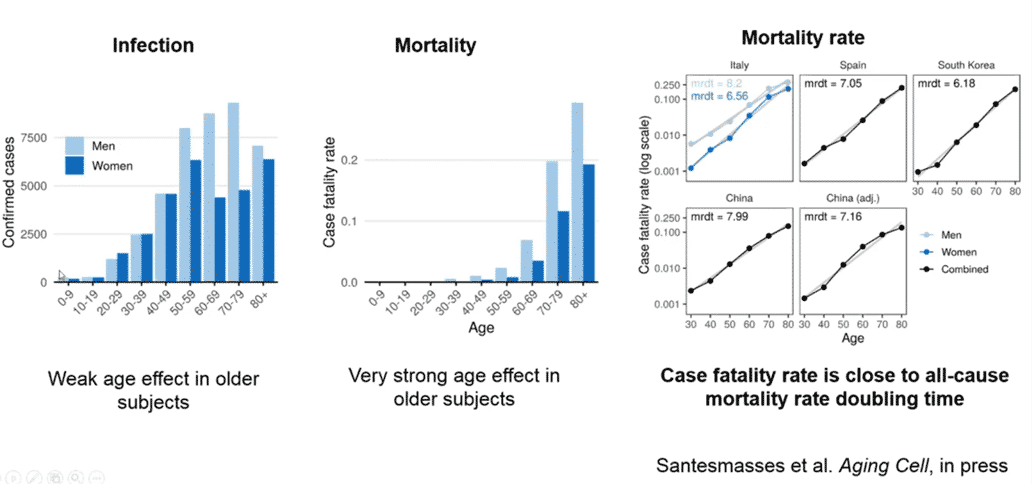
\includegraphics[width=\textwidth]{corona_death_rates} \\
    Source: \cite{10.1111/acel.13230}
\end{frame}


\begin{frame}[c]{All Deaths correlate with Age}
    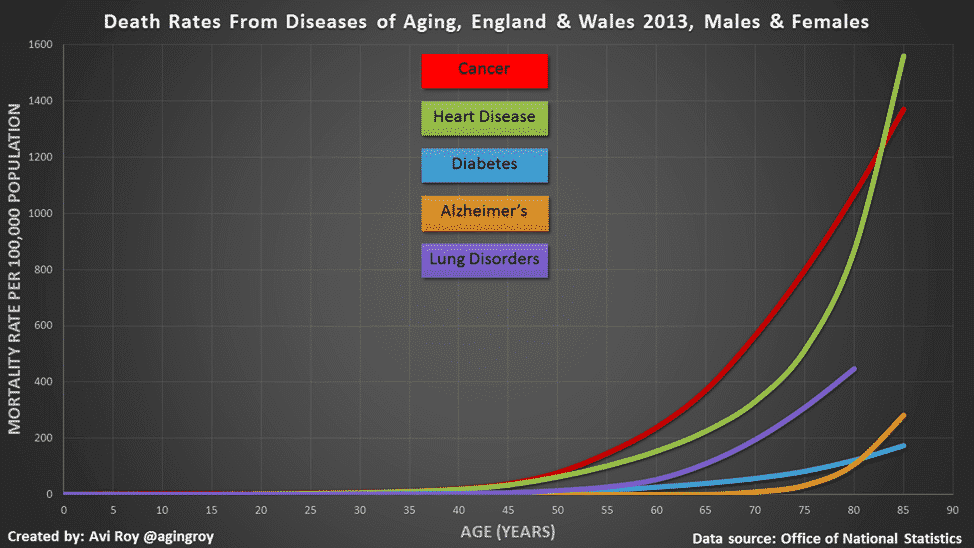
\includegraphics[width=\textwidth]{death_rates}
    % Picture with death likelihood by cause and age \\
    % Conclusion: People die from age, not by other causes
\end{frame}


\begin{frame}[c]{Very real Potential in Comparison}
    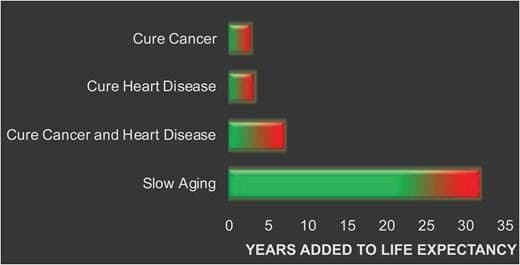
\includegraphics[width=\textwidth]{potential}
    Source: \cite{10.1093/ppar/prz022}
\end{frame}



\section{Is aging necessary?}


\begin{frame}[c]{Animals that don't age}
    \large
    \begin{itemize}[<+(1)->]
        \item hydra (biologically immortal) \cite{martinez1998mortality}
        \item naked mole rats \cite{ruby2018naked}
        \item tortoises \cite{miller2001escaping}
        % \item whales
        \item some sharks \cite{Greenlan67:online}
        \item some clams \cite{munro2012extreme}
    \end{itemize}
\end{frame}

\begin{frame}[c]{Senolytics}
    Objection: but it's natural \\
    (or: there is no way it could work) \\
    Examples of old animals: \\
    
    \begin{itemize}[<+(1)->]
        \item sharks
        \item moles
        \item others
        \item and many more
    \end{itemize}
    Conclusion: it's not natural
\end{frame}



\begin{frame}[c]{Studies with Mice}
    and how much life got extended: living twice as long QUALY is possible
\end{frame}

% \section{What is aging?}


\subsection{Definition and Hallmarks}

\begin{frame}[c]{Aging}
    \large

    \begin{block}{Definition}
        Aging is characterized by progressive decline in tissue and organ
        function and increased risk of mortality. From \cite{sen2016epigenetic}
    \end{block}
    \pause
    But how can we measure it?
\end{frame}


\begin{frame}[c]{Hallmarks of Aging}
    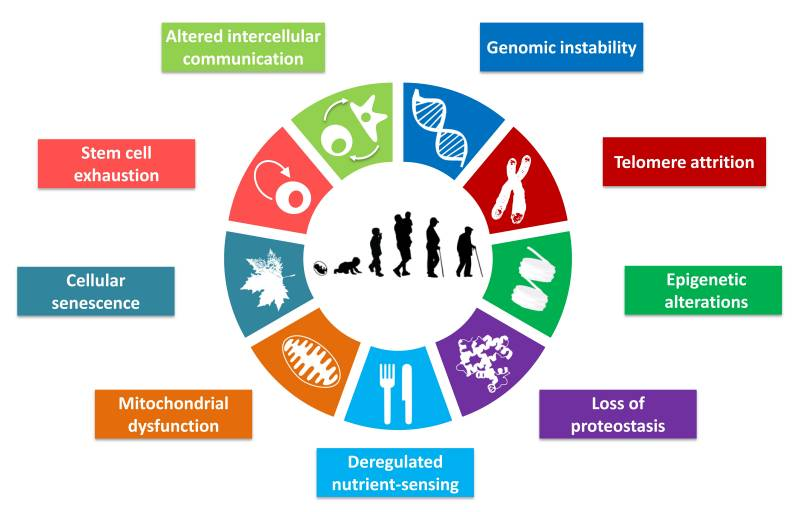
\includegraphics[width=\textwidth]{hallmarks_aging} \\
    \cite{lopez2013hallmarks}
    % \begin{itemize}[<+(1)->]
    %     \item Genomic instability
    %     \item Telomere attrition
    %     \item Epigenetic alterations
    %     \item Loss of proteostasis
    %     \item Deregulated nutrient-sensing
    %     \item Mitochondrial dysfunction
    %     \item Cellular senescence
    %     \item Stem cell exhaustion
    %     \item Altered intercellular communication
    % \end{itemize}
\end{frame}




% \section{How can we Slow down Aging?}

\subsection{Overview}

\begin{frame}[c]{Goal of Anti-Aging Research}
    \large
    As I understand it, the goal of anti-aging research is \textbf{the extension of the human lifespan}.

    Ideally by stopping aging or achieving neglegible senescence.
    Intermediate goals include slowing down aging, and increasing QUALYs
    (QUality-Adjusted-Life-Years).
    \pnote{
        neglegible senescence = not aging biologically \\
        \par
        neglegible senescence is further out, we are \\
        barely able to slow it down a few percent \\
        \par
        aim for longevity escape velocity
    }
\end{frame}

\begin{frame}[c]{Potential Strategies to Slow down Aging}
    \scriptsize
    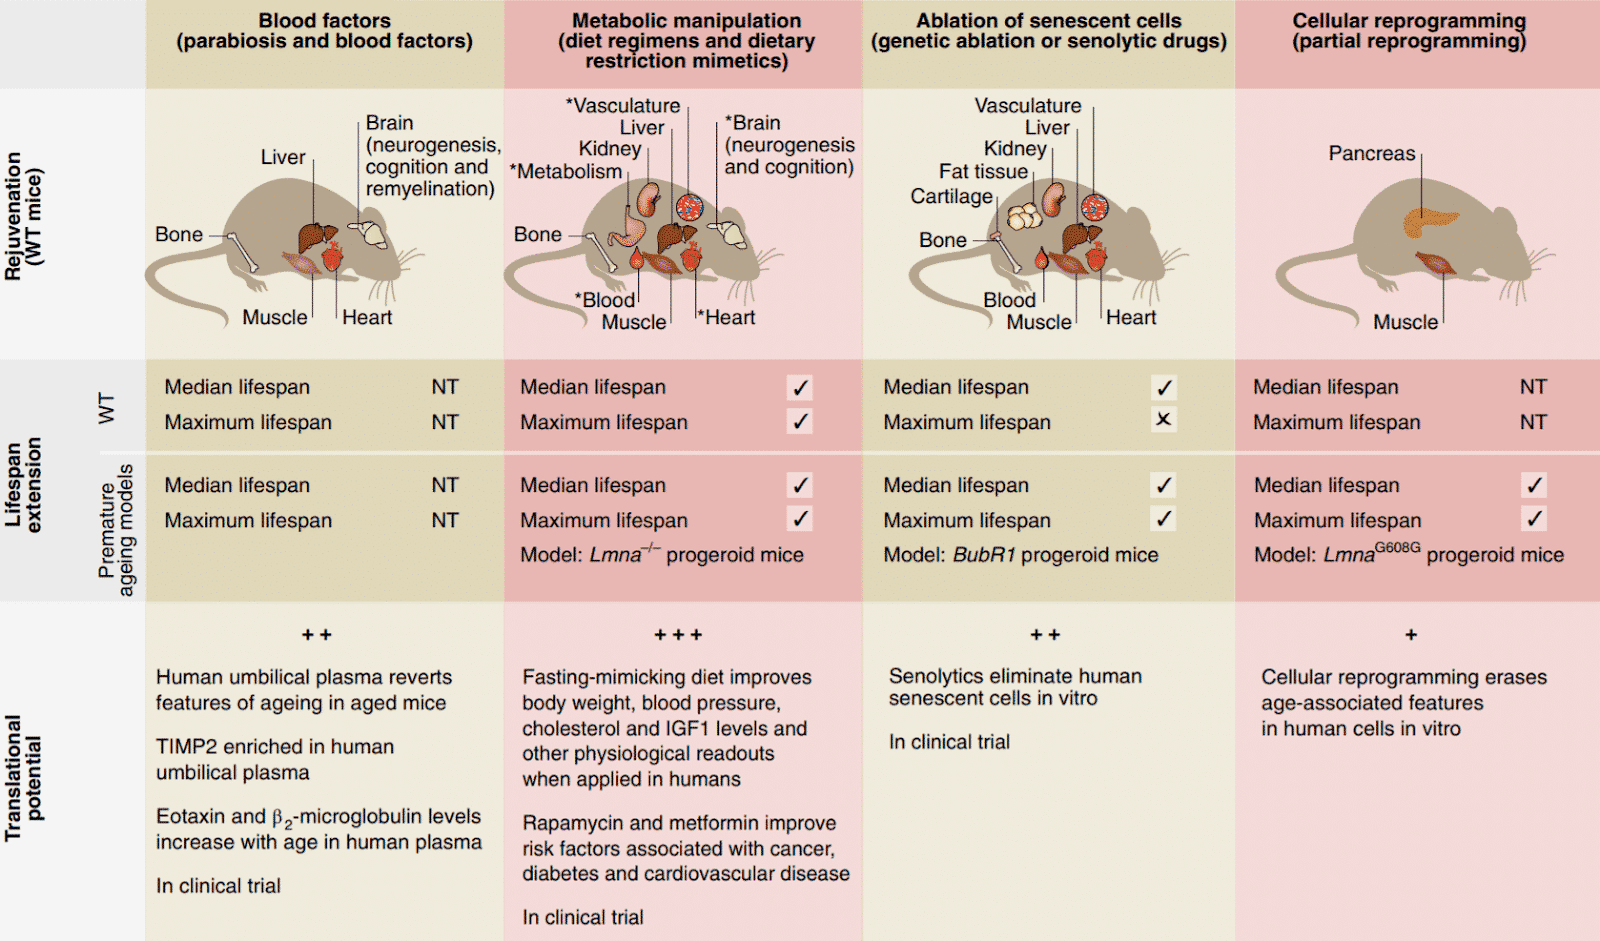
\includegraphics[width=\textwidth,clip,trim=0 280 0 0]{strategy_comparison_short} \\
    Source: \cite{mahmoudi2019turning}, picture modified

    \pnote{
        Comparison of rejuvenation strategies \\
        Currently highest potential, but more exist
        \par
        We will take a deeper look at all of them \\
        No need to study overview for long
        \par
        Treatment initiated midlife or later \\
        \par
        Next: Parabiosis
    }
    % go real in-depth on two topics, don't spread too much
    % remove parabiosis and either cellular reprogramming (since epigenetics first) or senolytics

    % \pnote{A comparison of the four emerging rejuvenation strategies: blood factors,
    % metabolic manipulation, ablation of senescent cells and cellular
    % reprogramming. The figure depicts the features that improve when treatment
    % in mice is initiated at midlife or later. The top panel shows organs or
    % tissues that exhibit a rejuvenated phenotype in wild-type (WT) mice. For
    % rapamycin, features that have been shown to improve also in young mice
    % following treatment are indicated with an asterisk (*). The effect on
    % lifespan, proposed primary mode (or modes) of action and possible
    % trade-offs of these strategies are also presented. Finally, the
    % translational potential in humans is indicated by the increasing number of
    % plus signs (+) based on present evidence in human ageing and current
    % feasibility. NT, not tested. Question marks indicate possible modes of
    % action and trade-offs.}
\end{frame}



\subsection{Metabolic Manipulation}

\begin{frame}[c]{Dietary Restriction in D. melanogaster (Fruit Fly)}
    \scriptsize
    % trim = l b r t
    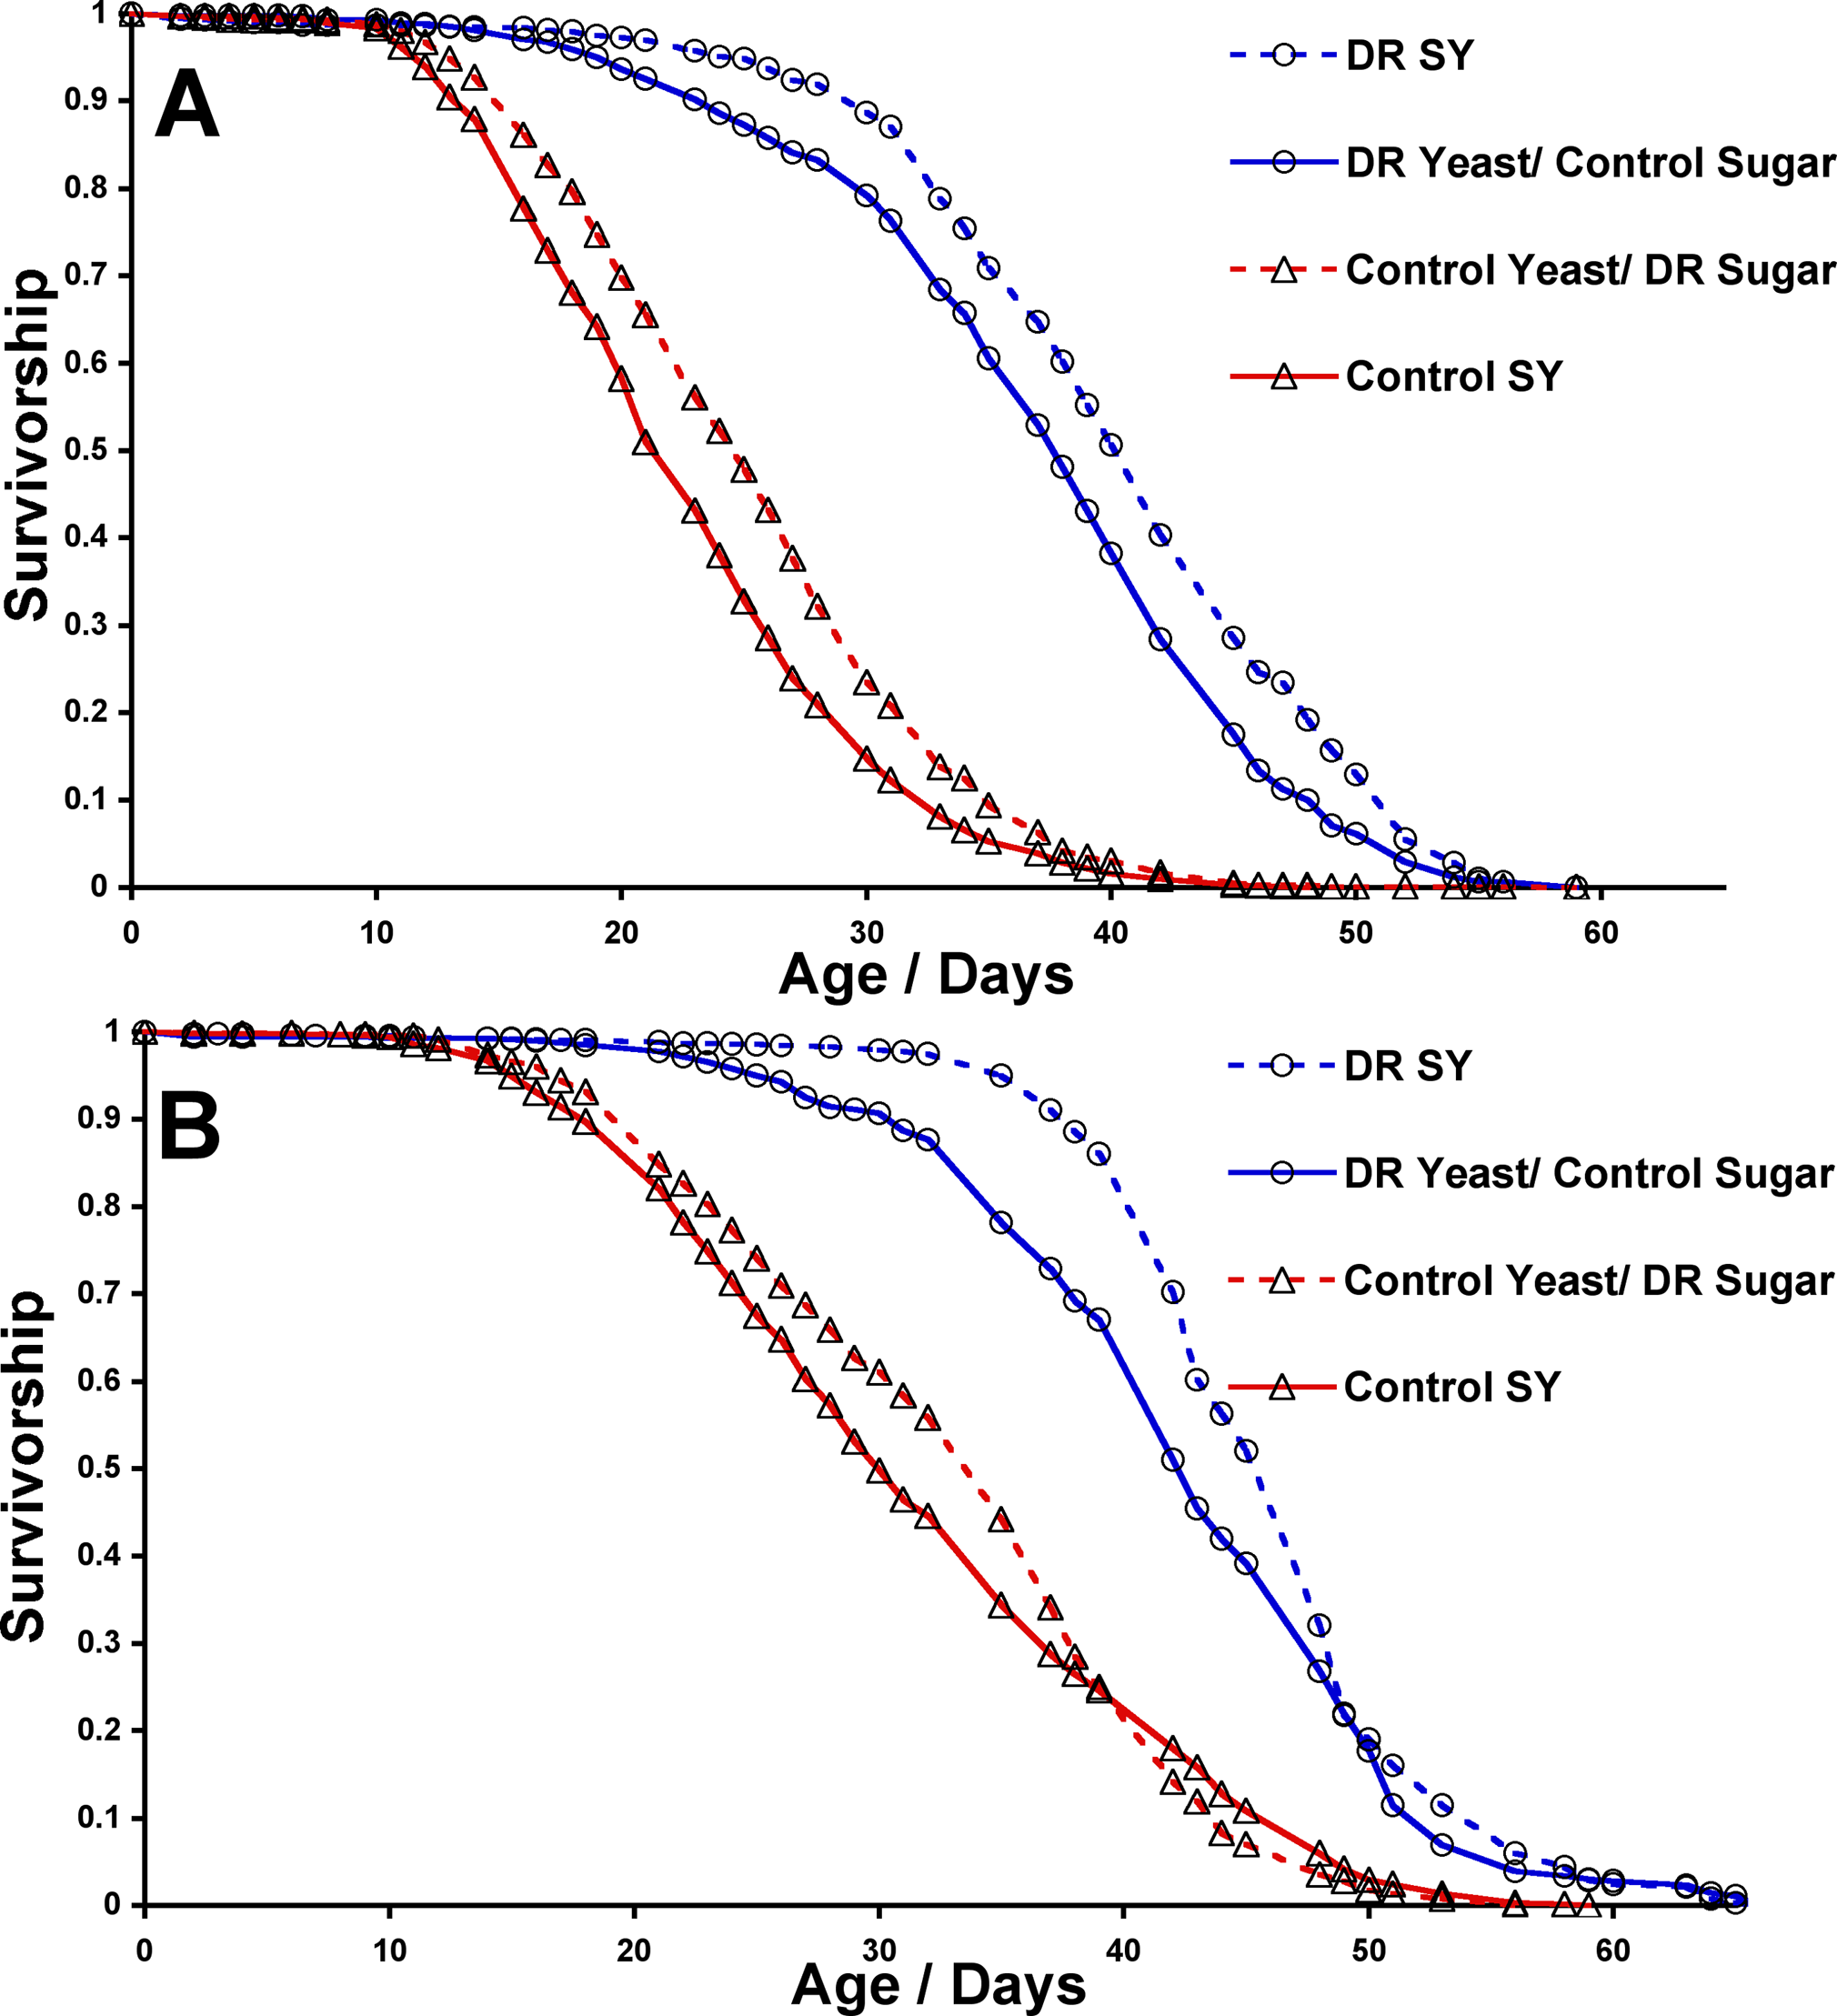
\includegraphics[width=\textwidth,clip,trim=0 57 0 0]{cr_lifespan_increase} \\
    Source: \cite{mair2005calories}
    \small
    \begin{multicols}{2}
    \begin{itemize}
        \item DR = Dietary Restriction
        \item Control = No Restriction
        \item S = Sugar
        \item Y = Yeast
    \end{itemize}
    \end{multicols}
    \pnote{
        Originally caloric restriction \\
        Experiment showed: not just calories \\
        Has been replicated as well \\
        Lifespan increase 20-40\% \\
        A/B replication of same setup
        \par
        Visible: does not just depend on calories \\
        Also well-established in Humans
        \par
        Next: Why does this work? What does it do? \\
    }
\end{frame}


\begin{frame}[c]{Dietary Restriction Effects}
    \large
    \begin{itemize}[<+(1)->]
        \item 'Different' mitochondrial energy production (less Reactive Oxygen Species, ROS)
        \item Reduced protein synthesis and DNA duplication
        \item Increased repair capacity (SIRT and others)
        \item Increased removal of misfolded proteins (Autophagy)
        \item Reduced inflammation and proliferation
    \end{itemize}
    \pause
    Overall: Optimizing energy and resource usage
    \pnote{
        ROS = Reactive Oxygen Species, damage-inducing \\
        Usual mode: just blast through / press ahead \\
        "Ohne Rücksicht auf Verluste" \\
        Less safety checks and enthusiastic production
        \par
        Works, as usually enough energy is present \\
        Also: Mitochondrial downregulation \\
        Proliferation: cell division and protein synthesis
        \par
        Maybe we can target these pathways directly? \\
        Next: Inhibiting mTOR receptors
    }
\end{frame}



\begin{frame}[c]{Metformin Effects}
    \scriptsize
    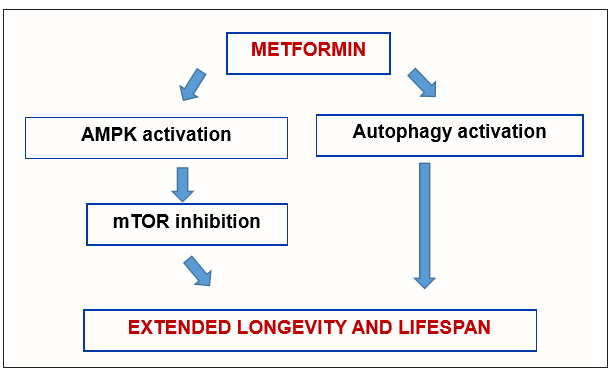
\includegraphics[width=\textwidth]{metformin_effects} \\
    Source: \cite{podhorecka2017metformin}
\end{frame}

\begin{frame}[c]{Method Evaluation: Metabolic Manipulation}
    \textbf{Hallmarks affected}: \\
    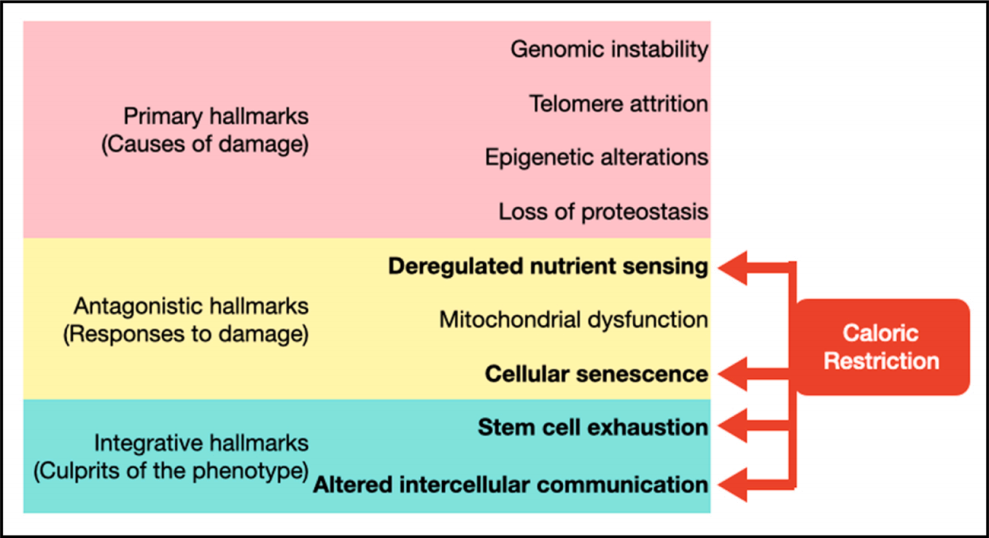
\includegraphics[width=0.7\textwidth]{cr_pathway_effects}
    % \begin{itemize}[<+(1)->]
    %     \item Deregulated Nutrient Sensing
    %     \item Cellular Senescence
    %     \item Stem Cell Exhaustion
    %     \item Altered Intercellular Communication
    % \end{itemize}
    \scriptsize
    Source: \cite{erbaba2020effects} \\
    \normalsize
    \pause
    Lifespan extension: about 20-40\% QUALY \cite{swindell2012dietary} \\
    \pause
    \textbf{State: In clinical trial}, e.g. \cite{TAMETarg47:online}
    \pnote{
        More of a 'slow down', preventing worst case \\
        Not silver bullet, rather 'one-trick pony' \\
        Not clear that this is correct classification
        \par
        Not 'root-cause' prevention \\
        but still amazing progress \\
        \par
        Next: Senolytics
    }
\end{frame}


\subsection{Senolytics}

\begin{frame}[c]{Senescent Cells: What are they?}
    \large
    \begin{itemize}[<+(1)->]
        \item `Zombie-like death-resistent cells'
        \item Old or (partially) damaged cells
        \item Sending out Senescence-Associated Secretory Phenotype (SASP)
        \item SASP disrupts intercellular communication, causing inflammation and age-related diseases
        \item Cells manage to induce apoptosis (cell-suicide) or get removed by the immune system
        \item About 8\% of cells in young, and 17\% of cells in old mice are senescent \cite{folgueras2018mouse}
    \end{itemize}
    \pnote{
        SASP part of damage-fallback state \\
        'I won't be able to fix this' \\
        Severely disrupts intercellular communication
        \par
        Very interesting: senescent difference \\
        in old vs young mice \\
        \par
        Next: Senolytics Effects
    }
\end{frame}


% \begin{frame}[c]{Senescent Cell Effects}
%     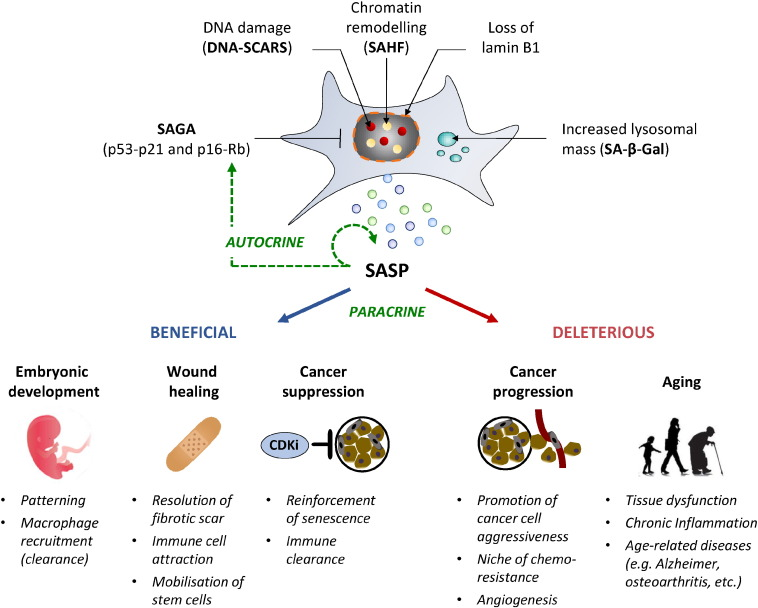
\includegraphics[height=0.85\textheight]{sasp_effects} \\
%     Source: \cite{malaquin2016keeping}
%     \pnote{
%         SASP meant to increase cell-turnover \\
%         more apoptosis, more cell growth to replace \\
%         less 'safety checks' with high proliferation
%         \par
%         also toxic agents + ROS to make less hospitable \\
%         specific factors induce cell death and growth
%         \par
%         good for wound healing (high turnover) \\
%         Klassisch: 'Entzündung' (inflammation)
%         \par
%         Next: Senolytic Uses and Effects
%     }
% \end{frame}


% \begin{frame}<handout>[c]{Inflammation Effects}
%     \begin{aquote}{\cite{NintilTh68:online}}
%         {\em Also, the environment that inflammation creates is one that is} meant to
%         increase cell turnover {\em (More apoptosis, but also more cell growth to
%         replace lost cells), with granulocytes secreting toxic agents
%         (Including ROS) to make the area affected less hospitable (But also
%         increases damage to DNA), and specific cytokines like the} tumor
%         necrosis factor that induce cell death, and growth factors that promote
%         cell growth.
%     \end{aquote}
% \end{frame}


\begin{frame}[c]{Senolytics and Aged Cells}
    \scriptsize
    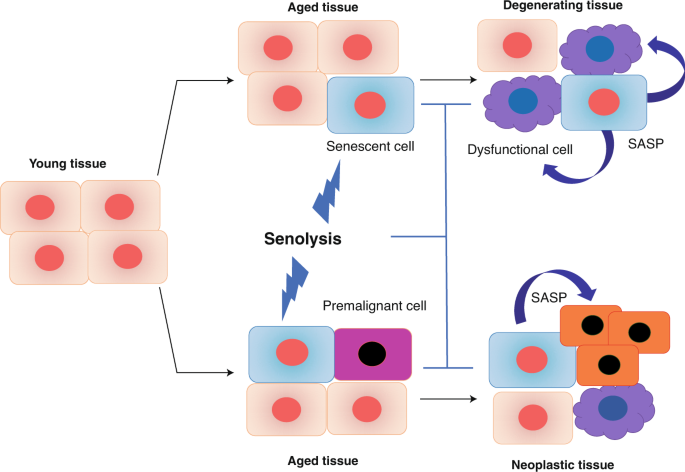
\includegraphics[height=0.85\textheight]{senolytics_effect}
    Source: \cite{dolgin2020send}
    \pnote{
        SASP has negative effects on neighbouring cells \\
        disrupting intercellular communication \\
        ground for cell-turnover -> tumorgenesis \\
        awesome machanism for healthy tissue!
        \par
        Senolytics 'help Senescent cells to die' \\
        (euthanasia) or modulate SASP damage
        \par
        Next: Senolytics Evaluation
    }
\end{frame}

% \begin{frame}[c]{Senolytics (Drugs killing senescent cells)}
%     Senescent cells are a kind of 'zombie'-like cell that accumulate with age. They are death-resistant cells that secrete proinflammatory factors associated with a range of age-related diseases (below, right):

% Cellular senescence is associated with multiple human disorders. The development of galactose‐conjugated and fluorescent probes to detect and highlight senescent cells offers an important opportunity for longitudinal monitoring of senescence in clinical trials. Pharmacologically active small compounds known as senolytics inhibit pro‐survival pathways in senescent cells leading to apoptosis, a therapeutic strategy that may additionally be enhanced by the use of immune modulators promoting natural clearance of senescent cells. Finally, nanoparticles encapsulating cytotoxic drugs, tracers and/or small molecules can be used as theranostic tools, both for therapeutic and diagnostic purposes. Source: here
% There are various strategies being explored to kill or reprogram senescent cells (above, left), including senolytics. Senolytics are drugs that kill senescent cells to improve physical function and healthy lifespan. When administered to older mice, senolytics have been shown to reverse many aspects of aging such as cataracts, and arthritis (below):

% Killing senescent cells with senolytics extends the median healthy lifespan by up to 27\% in mice (below). Several senolytics, such as the combination of dasatinib and quercetin, and fisetin are in clinical trials in humans today.

% Study design for clearance of senescent cells mouse cohort. Median survival (in days, d) and percentage increase in median survival are indicated. Source: here
% Hallmarks of aging reversed: senolytics decelerate cellular senescence, improve epigenetic markers and restore intercellular communication (by reducing inflammation associated with senescent cells) to extend healthy lifespan.
% \end{frame}


\begin{frame}[c]{Method Evaluation: Senolytics}
    \textbf{Hallmarks affected}: \\
    \begin{itemize}[<+(1)->]
        \item Decelerate Cellular Senescence
        \item Improve Epigenetic Markers
        \item Restore Intercellular Communication (by reducing inflammation associated with senescent cells)
    \end{itemize}
    \pause
    Lifespan extension: 27\% median Life\\
    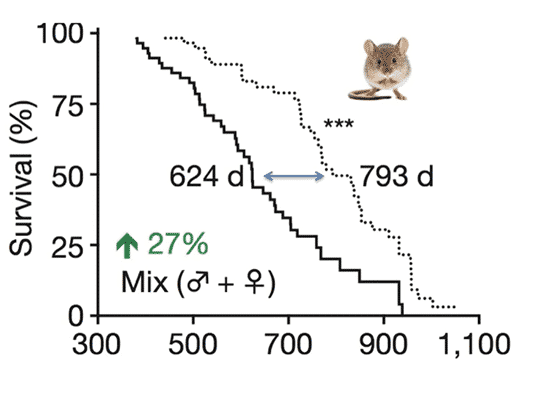
\includegraphics[width=0.4\textwidth]{senolytics_extend_life}
    \scriptsize
    Source: \cite{baker2016naturally} \\
    \normalsize
    \pause
    \textbf{State: In clinical trial}
    \pnote{
        Going much more in on root causes \\
        Depends heavily on immune system capacity \\
        \par
        Bonus: Very different mechanism, \\
        so probably good complement to other methods \\
        \par
        Next: Cellular Reprogramming
    }
\end{frame}


\subsection{Other Approaches}

\begin{frame}[c]{Other Promising Approaches}
    \large
    \begin{itemize}[<+(1)->]
        \item Blood Exchange (Parabiosis) \cite{conese2017fountain}
        \item Cellular Reprogramming \cite{ocampo2016vivo}
        \item Thymic (Immune System) rejuvenation \cite{fahy2019reversal}
        \item Sirtuin activation for DNA repair \cite{mohar2012sirtuin}
        % \item Boosting mitochondrial function with NAD+ precursor molecules \cite{aman2018therapeutic}
        % \item Identifying genetic Markers \cite{kenyon2010genetics}
        \item Many more ...
    \end{itemize}
    \pnote{
        SIRT are part of DNA damage repair pathways \\
        NAD is being consumed in emergency response \\
        NAD = Nicotinamide adenine dinucleotide \\
        Preventing dangerous mitochondrial fail-states \\
        Unclear how genetic markers affect longevity
        \par
        Next: Evaluation
    }
\end{frame}


% \begin{frame}[c]{Method Evaluation: Other Approaches}
%     \large
%     \textbf{Hallmarks affected}: ??? \\
%     \pause
%     Lifespan extension: Most 5\%-40\% \\
%     \pause
%     State: Active research, some in animal or clinical trials
%     \pnote{
%         A lot of different approaches \\
%         Many with as-yet-unknown effects on vertebrates \\
%         yet others already in clinical trials \\
%         All of what I'm presenting is active research
%         \par
%         Ask me about state of yeast
%         \par
%         Next: What can I do?
%     }
% \end{frame}

% \section{What can I do?}

\subsection{Pharmacological}

\addtocounter{framenumber}{1}
\begin{frame}[standout]
    \LARGE
    This is NOT Medical Advice!
\end{frame}

\begin{frame}[c]{Pharmacological}
    List of medications taken regularly by anti-aging researchers:

    \begin{itemize}[<+(1)->]
        \item Metformin - calorie restriction mimetic that controls blood sugar
            % ist in deutschland diabetes typ2 medikament: erste wahl
            % actually helpful for type 1 as well, but new knowledge
            % vorteil: hohe senkung von Hba1c-Wert (prozentual) (sollte bei gesund unter 6%, niedriger ist besser)
            % -> verschreibungspflichtig
            % nachteil: wirkmechamismus nicht vollständig bekannt
            %   hemmt glykosebildung (aus pyruvat) in leber
            %   seltene nebenwirkung: lactatacetose (lactat wird nicht zu zucker umgebaut), zu 50% tödlich
            % sehr potent, aber unklar wie viel es beim Menschen hilft
            % kritisch für Umwelt weil kann nicht abgebaut werden (verbrennen!)
            % hormonähnliche Wirkung, aber günstig: weniger als 1EUR/TAG
            % alternative: glieflocine (?) mit mehr vorteilen, aber viel teurer
        \item Quercetin - anti-aging flavenoid that acts as a senolytic
            % flavenoid: sekundäre pflanzenstoffe (z.B. Frost-, oder Lichtschutz)
            % hier: in Roter traube/Rotwein (teil Farbstoff) aber auch andere
            % 'soll antioxidativ wirken' (umstritten, insb. relevanz)
            % aber: wenig kommt an mit sehr kurzer wirkung, schwer wirkung nachzuweisen
            % verschreibungsfrei
        \item Resveratrol - sirtuin enzyme activator and calorie restriction mimetic
            % ähnlich einem flavonoid
            % verschreibungsfrei
        \item Vitamin D - blood tested to optimize, ideally 2000IU per day
            % meisten haben mangel, schadet nicht aufzufüllen
            % tatsächlich ein weitreichendes Hormon
            % 60-80μg/ml im Serum ideal, alles andere: erhöhtes sterblichkeitsrisiko
            % fettlösliches 'Vitamin', aber überdosierung enorm schwierig
            % bekommt man überall, billig
        \item Vitamin B12 - as many people are deficient
            % auch weit verbreiteter Mangel, organische substanz
            % tägl. bedarf: 2-3μg
            % insb. bei Fleischarmer Ernährung wichtig zu supplementieren
            % nur kleiner teil wird auch verwertet
            % bekommt man überall, billig
    \end{itemize}
\end{frame}


\begin{frame}[c]{Pharmacological II}
    On the more extreme end (for older people or people with a higher risk tolerance):

    \begin{itemize}[<+(1)->]
        \item Rapamycin - an mTOR inhibitor that attenuates senescence
            % immunsuppresiv
            % mTOR ist mega wichtig, hemmt proliferation aber auch immunabwehr (?)
            % wird nicht mehr eingesetzt
            % alternative: imatinib, auch mTOR-pfad-relatiert
            % auch nicht über verschreibungen, sehr teuer, gibt alternativen (auch teuer)
        \item NAD-boosters such as NMN (Nicotinamide) and NR - enhancers of stem cell function
            % NAD ist cofactor in versch. zeug (auch: Vit B2, D), hier: B3
            % bilden redox-cofactoren, zum elektronentransport, erlaubt sehr spezielle reaktionen
            % sirtruine konsumieren NAD, unklar wie viel das bringt
            % verschreibungsfrei, sehr günstig: Vit-B-Komplex (B2/B3) (alt: nur B3)

            % spermidin - soll telomerabbau verlangsamen (in vitro!)
            %   ist schon in gameten, unklar ob mehr hilft
            %   verschreibungsfrei, aber nicht sehr günstig
        \item Dasatinib - a senolytic usually used in combination with quercetin
            % auch mTOR-inhibitor
            % verschreibungspflichtig
    \end{itemize}
    % alles minimale effekte, viel wichtiger:
    % - gesunde & ausgewogene ernährung
    % - sport
    % - wenig stress
    % - keine depri
    \pause
    \LARGE
    \textbf{But: a balanced lifestyle will get you much further}
\end{frame}


\subsection{Lifestyle}

\begin{frame}[c]{Lifestyle is more important}
    \large
    Available medication can add only so much, much more important are:

    \begin{itemize}[<+(1)->]
        \item Healthy and balanced diet \cite{willcox2007caloric}
        \item Regular Exercise \cite{lee1995exercise}
        \item Low-Stress Environment
        \item Close friends \cite{olsen1991social}
        \item Fulfilling Life \cite{diener2011happy}
        \item Not suffering from depression \cite{cuijpers2002excess}
    \end{itemize}
    \pause
    The statistical evidence is clear on this!
\end{frame}

% \section{How can bioinformatics help?}

\subsection{Analysis}

\begin{frame}[c]{Analysis}
    Large datasets, ever-more data
\end{frame}


\begin{frame}[c]{Analysis}
    Will need new tools and software
\end{frame}

\subsection{Simulation}

\begin{frame}[c]{Simulation}
    current Pharmaceutical battle: better simulator
\end{frame}


\begin{frame}[c]{Simulation II}
    AlphaFold2 and others
\end{frame}


% '\include'
% - gives speed bonus when building, through caching in a seperate *.aux file
% - has a 'page break'
% - cannot be nested
% ------------- VS -------------
% '\input'
% - can be nested
% - does not have 'page breaks'
% - gives no caching benefit


%%%%%%%%%%%%%%%%%%%%%%%%%%%%%%%%%%%%%%%%%%%%%%%%%%%%%%%%%%%%%%%%%%%%%%%%%%%%%%%%%%%%%%%%%%%%%%%%%%%



%%%%%%%%%%%%%%%%%%%%%%%%%%%%%%%%%%%%%%%%%%%%%%%%%%SOURCES%%%%%%%%%%%%%%%%%%%%%%%%%%%%%%%%%%%%%%%%%%

\begin{frame}[c,fragile,allowframebreaks]{Sources}
\bibliographystyle{plainnat}
% \bibliographystyle{ieeetr}
\bibliography{references.bib}
\end{frame}

% \appendix
\backupbegin

\begin{frame}[c]{Rust: Code Example}
    \begin{codeboxed}{Code Example 1}
    \inputminted[linenos, fontsize=\normalsize]{Rust}{code/code_ownership.rs}
    \end{codeboxed}
\end{frame}

\begin{frame}[c]{Rust: Code Example}
    \begin{codeboxed}{Output Nr. 1}
        \footnotesize
        \verbatiminput{code/output1.txt}
    \end{codeboxed}
\end{frame}

\begin{frame}[c]{Rust: Code Example}
    \begin{codeboxed}{Code Example 2}
    \inputminted[linenos, fontsize=\normalsize]{Rust}{code/code_ownership2.rs}
    \end{codeboxed}
\end{frame}

\begin{frame}[c]{Rust: Code Example}
    \begin{codeboxed}{Output Nr. 2}
        \footnotesize
        \verbatiminput{code/output2.txt}
    \end{codeboxed}
\end{frame}

\backupend


\end{document}
